\section{Figuras}
\label{sec:figuras}


\begin{figure}[h]
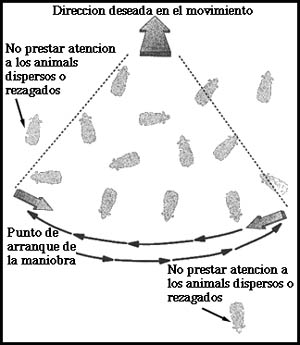
\includegraphics[scale=0.6]{figura111}\\
\centering
\caption{Técnica limpiaparabrisas}
\label{fig:figura111}
\end{figure}


\begin{figure}
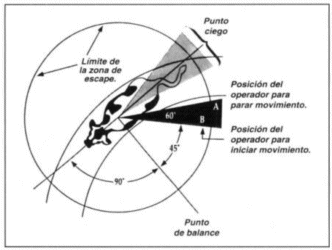
\includegraphics[scale=0.7]{figura112}\\
\centering
\caption{Zona de fuga}
\label{fig:figura112}
\end{figure}


\begin{figure}
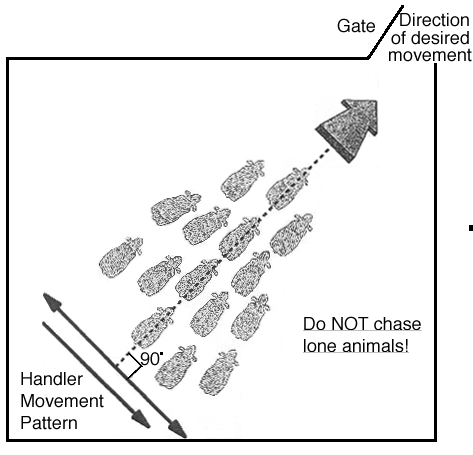
\includegraphics[scale=0.6]{figura113}\\
\centering
\caption{Sacar al ganado: Un controlador}
\label{fig:figura113}
\end{figure}


\begin{figure}
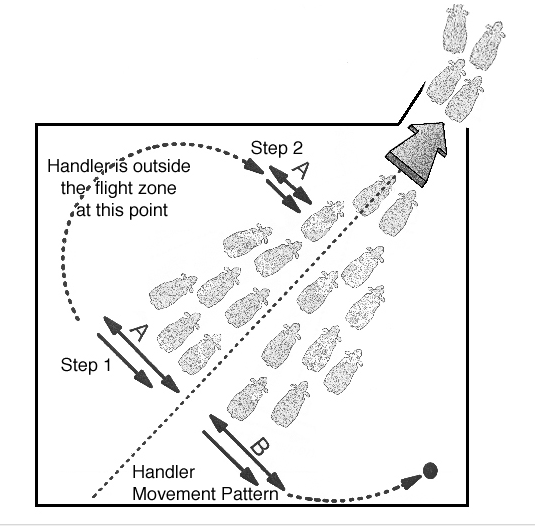
\includegraphics[scale=0.6]{figura114}\\
\centering
\caption{Sacar al ganado: Dos controladores}
\end{figure}


\begin{figure}
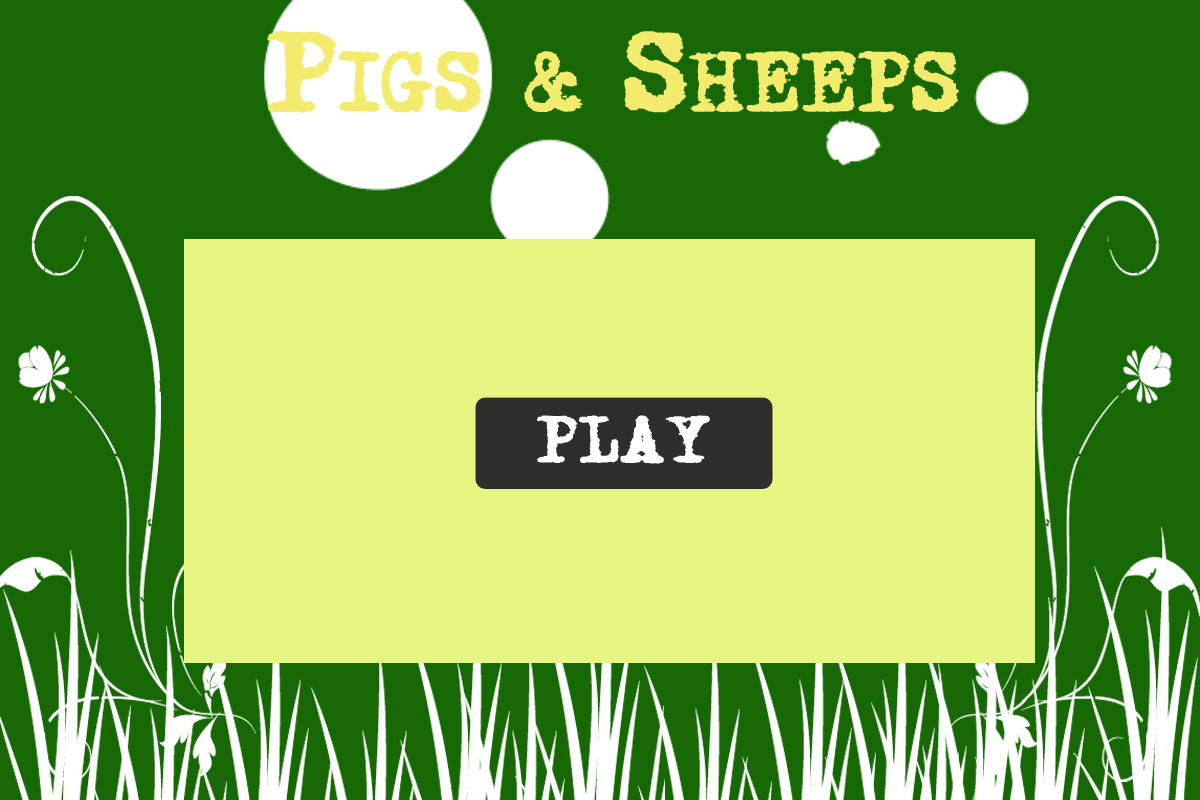
\includegraphics[scale=0.32]{figura311}\\
\centering
\caption{Primer diseño}
\end{figure}


\begin{figure}
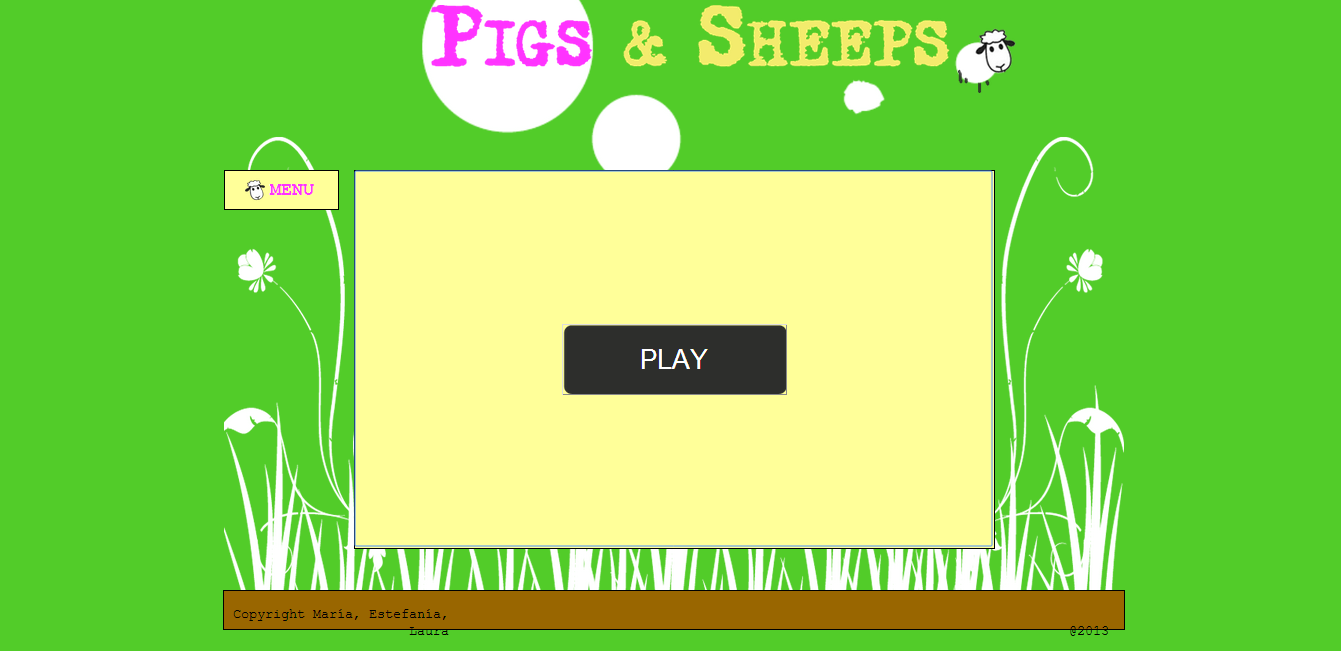
\includegraphics[scale=0.33]{figura312}\\
\centering
\caption{Segundo diseño}
\end{figure}


\begin{figure}
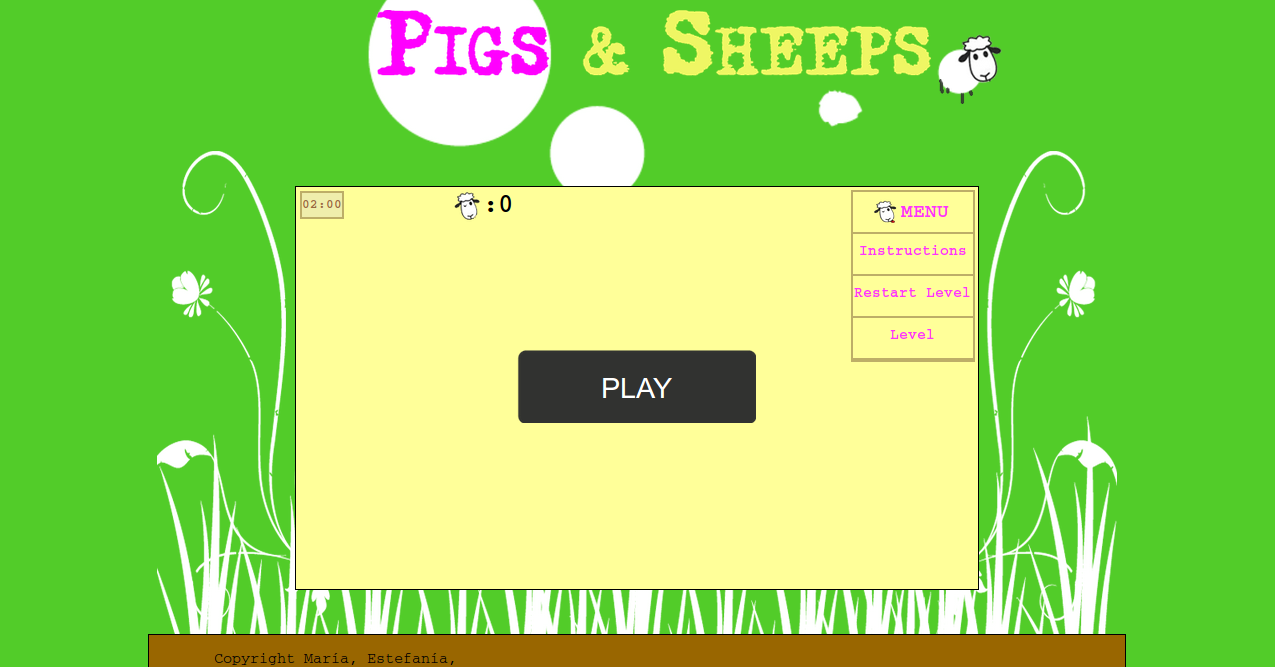
\includegraphics[scale=0.33]{figura313}\\
\centering
\caption{Diseño final}
\end{figure}


\begin{figure}
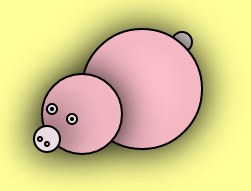
\includegraphics{figura321}\\
\centering
\caption{Primer cerdito}
\end{figure}


\begin{figure}
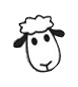
\includegraphics{figura322}\\
\centering
\caption{Oveja - sólo cabeza}
\end{figure}


\begin{figure}
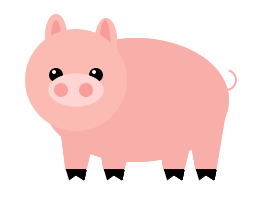
\includegraphics{figura323}\\
\centering
\caption{Cerdito definitivo}
\end{figure}


\begin{figure}
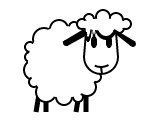
\includegraphics{figura324}\\
\centering
\caption{Oveja definitiva}
\end{figure}


\begin{figure}
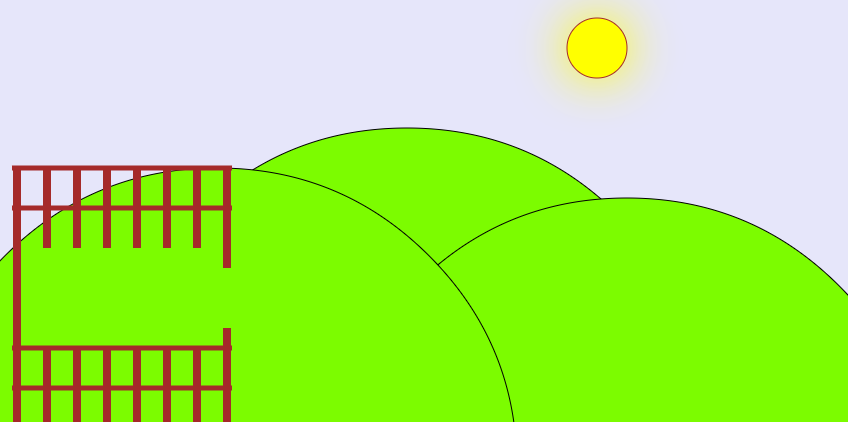
\includegraphics[scale=0.33]{figura325}
\centering
\caption{Primer canvas}
\end{figure}


\begin{figure}
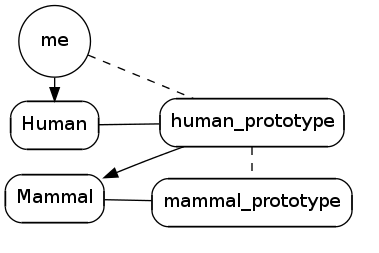
\includegraphics[scale=0.6]{figura413}\\
\centering
\caption{Herencia prototípica}
\end{figure}


\begin{figure}
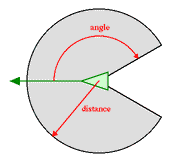
\includegraphics{figura4212}\\
\centering
\caption{Oveja. Cabeza}
\end{figure}

 
\begin{figure}
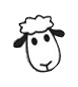
\includegraphics{figura322}\\
\centering
\caption{gráfico de velocidades y aceleraciones}
\end{figure}


\begin{figure}[h!]
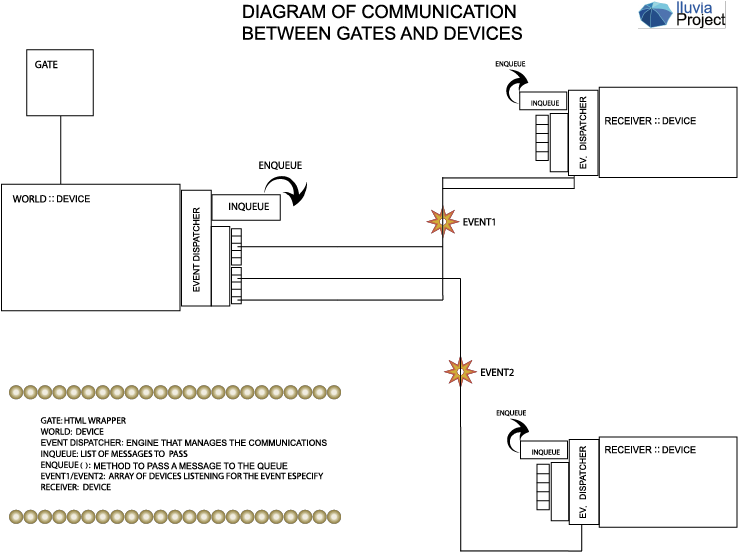
\includegraphics[scale=0.6]{figura511}\\
\centering
\caption{Diagrama Gate y Devices}
\end{figure}

